\begin{frame}{Reactive walking pattern generation}
\framesubtitle{Example :}
  \begin{center}
  \scalebox{0.8}{
	\newcommand{\tetazero}{20.55}
	\newcommand{\Fkxzero}{-20}
	\newcommand{\Fkyzero}{20}
	
	\newcommand{\tetaone}{-20}
	\newcommand{\Fkxone}{5}
	\newcommand{\Fkyone}{0}
	
	\newcommand{\tetatwo}{20}
	\newcommand{\Fkxtwo}{25}
	\newcommand{\Fkytwo}{20}
	
	
	\definecolor{color1}{RGB}{1, 121, 111}% corail
	\definecolor{color2}{RGB}{27, 79, 8}% orange 
	\definecolor{color3}{RGB}{237 , 127 ,16}%
	\definecolor{color4}{rgb}{0.9,0.,0.}	
	\begin{tikzpicture}
		\begin{axis}[xlabel=x,ylabel=y,xmin=-0.2,xmax=0.6,ymin=-0.25,ymax=0.35]
			\only<1>{
			 \addplot[black,thick=2pt,fill=gray!20]
          table{../figures/images/tikz/footstartright.dat};
			}
			\only<1-2>{
        \addplot[black,thick=2pt,fill=gray!20]
          table{../figures/images/tikz/footstartleft.dat};       
			}
			\only<2-3>{
        \addplot[black,thick=2pt,fill=gray!20]
          table{../figures/images/tikz/foot2.dat};
      }
      \only<3-4>{
        \addplot[black,thick=2pt,fill=gray!20]
          table{../figures/images/tikz/foot3.dat};
      }
      \only<4-5>{
        \addplot[black,thick=2pt,fill=gray!20]
          table{../figures/images/tikz/foot4.dat};
			}
			\only<5-6>{
        \addplot[black,thick=2pt,fill=gray!20]
          table{../figures/images/tikz/footendleft.dat};
			}
			\only<6>{
        %\addplot[black,thick=2pt,dashed,fill=white,opacity=0.5]
        \addplot[black,thick=2pt,fill=gray!20]
          table{../figures/images/tikz/footendright.dat};
			}
	    \only<9->{
			  \addplot[black,thick=5pt,fill=gray!20]
			    	table{../figures/images/tikz/footconstraint.dat}; 
  			  \addplot[dashed,black,thick=5pt,fill=gray!20]
			    table{../figures/images/tikz/foot.dat};
			  \addplot[black,very thick,fill=gray!20]
			    table{../figures/images/tikz/footmargin.dat};
	    }
	    	\only<7-8>{
	    	  \addplot[dashed,black,thick=2pt,fill=gray!10,opacity=0.5]
          table{../figures/images/tikz/footstartright.dat};
        \addplot[dashed,black,thick=2pt,fill=gray!10,opacity=0.5]
          table{../figures/images/tikz/footstartleft.dat};
        \addplot[dashed,black,thick=2pt,fill=gray!10,opacity=0.5]
          table{../figures/images/tikz/foot2.dat};
        \addplot[dashed,black,thick=2pt,fill=gray!10,opacity=0.5]
          table{../figures/images/tikz/foot3.dat};
        \addplot[dashed,black,thick=2pt,fill=gray!10,opacity=0.5]
          table{../figures/images/tikz/foot4.dat};
        \addplot[dashed,black,thick=2pt,fill=gray!10,opacity=0.5]
          table{../figures/images/tikz/footendleft.dat};
        \addplot[dashed,black,thick=2pt,fill=gray!10,opacity=0.5]
          table{../figures/images/tikz/footendright.dat};
	    	}
	    	\only<8->{
			  % com
			  \addplot[color1,thick=2pt] table[x index= 0,y index=1]
			    	{../figures/images/tikz/table.dat};
			}
	    	\only<7->{
	      % cop
			  \addplot[color2,thick=5pt] table[x index= 2,y index=3]
			    	{../figures/images/tikz/table.dat}; 
			}
		\end{axis}
	\end{tikzpicture}
	}
	\end{center}
\end{frame}


\begin{frame}{Reactive walking pattern generation \only<4>{with obstacles}}
  \begin{minipage}{0.48\textwidth}
    Optimization problem solved :
    \vspace*{-0.3cm}
    \begin{equation*}
      \begin{aligned}
        \min_{{\bf U}_k} 
        \sum_{i=0}^{j=4} w_i L_i({\bf U}_{k}) & \\
        {\bf X}_{k+1} = {\bf A}{\bf X}_{k} + {\bf B} {\bf U}_k & \\
        \underline{\bf P} < {\bf P}\only<4>{{\color{red}{({\bf U}_k)}}} {\bf U}_k  < \overline{\bf P}& \\
      \end{aligned}
    \end{equation*}
    with ${\bf U}_k=\begin{pmatrix} \dddot{\bf C}^x_k \; {\bf F}^x_k\; \dddot{\bf C}^y_k \;{\bf F}^y_k \;\only<4>{\color{red}{{\bf F}^{\theta}_k}}\end{pmatrix}^T$ \\
  \end{minipage}
  %
  \begin{minipage}{0.48\textwidth}
    \only<1-3>{
      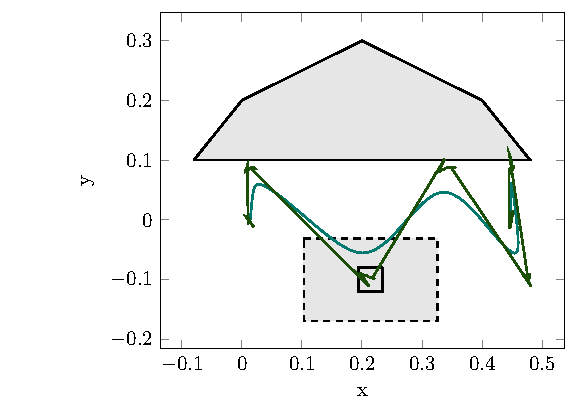
\includegraphics[width=\textwidth]{./images/tikz/convexHulls2}
    }
    \only<4>{
      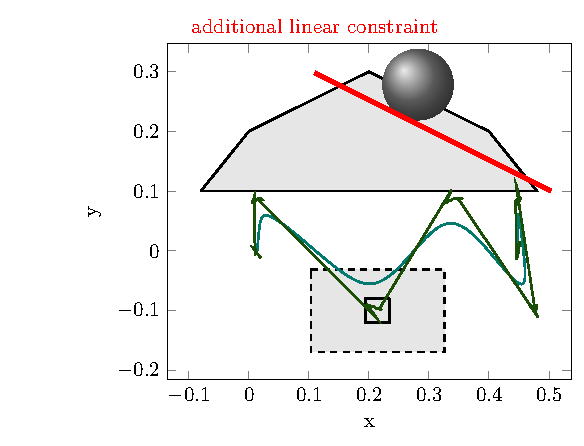
\includegraphics[width=\textwidth]{./images/tikz/convexHullsplusObstacles2}
    }
  \end{minipage}\\

  $\dddot{\bf C}_k$ = CoM jerk ; ${\bf F}_k$ = Support Foot Position\\
  \begin{center}
  \only<1>{
    {
       $L_1({\bf U}_k)$ : linear velocity tracking
%      \begin{equation*}
%        \text{linear velocity tracking : }
%        L_1({\bf U}_k) = \lVert \dot {\bf X}_{k} - {\bf X}_{k}^{ref} \rVert^2_2
%        +  \lVert \dot {\bf Y}_{k} - {\bf Y}_{k}^{ref} \rVert^2_2 
%      \end{equation*}
    }
  }
  \only<2>{
    {
       $L_2({\bf U}_k)$ : control norm
%      \begin{equation*}
%        \text{control norm : }
%        L_2({\bf U}_k) = \lVert \dddot {\bf X}_{k} \rVert^2_2
%        + \lVert \dddot {\bf Y}_{k} \rVert^2_2
%      \end{equation*}
    }
  }
  \only<3>{
    {
       $L_3({\bf U}_k)$ : balance criteria
%      \begin{equation*}
%        \text{balance criteria : }
%        L_3({\bf U}_k) = \lVert {\bf X}_{k}^{f} - CoP_{k+1}^{x} \rVert^2_2 +
%        \lVert {\bf Y}_{k+1}^{f} - CoP_{k+1}^{y} \rVert^2_2 
%      \end{equation*}
    }
  }
  \only<4>{
    {
       $L_4({\bf U}_k)$ : angular velocity tracking
%      \begin{equation*}
%        \text{angular velocity tracking : }
%        L_4({\bf U}_k) = \lVert {\bf \Theta}_{k} 
%        - \int {\bf \Theta}_{k}^{ref} dt \; \rVert_2^2 
%    \end{equation*}
    }
  }
  \end{center}
  
\end{frame}

%%%%%%%%%%%%%%%%%%%%%%%%%%%%%%%%%%%%%%%%%%%%%%%%%%%%%%%%%%%%%%%%%%%%%%%%%%%%%%%


\begin{frame}{SQP Solver}

\begin{itemize}
\item Principle
\begin{itemize}
\item Original nonlinear problem, free variable : ${\color{txtcolor2}{\bf U}_k}$
\item Taylor approximation, creation of a sequence of QP,
      
      free variable : ${\color{txtcolor5}{\bf \Delta U}_k}$
\end{itemize}
\end{itemize}

\begin{itemize}
\item Observation : $1$ iteration is enough to solve the original QP

[Herdt Advanced Robotics 2010].
\item Hypothesis : $1$ optimal solution of a QP is enough to solve the SQP.
\item Statistical results : mean $1.2$ optimal solution of a QP is enough to solve the SQP.
\end{itemize}

\end{frame}

%%%%%%%%%%%%%%%%%%%%%%%%%%%%%%%%%%%%%%%%%%%%%%%%%%%%%%%%%%%%%%%%%%%%%%%%%%%%%%%

\begin{frame}{Experiment on HRP2}
  \begin{center}
    \movie[autostart,loop]{
    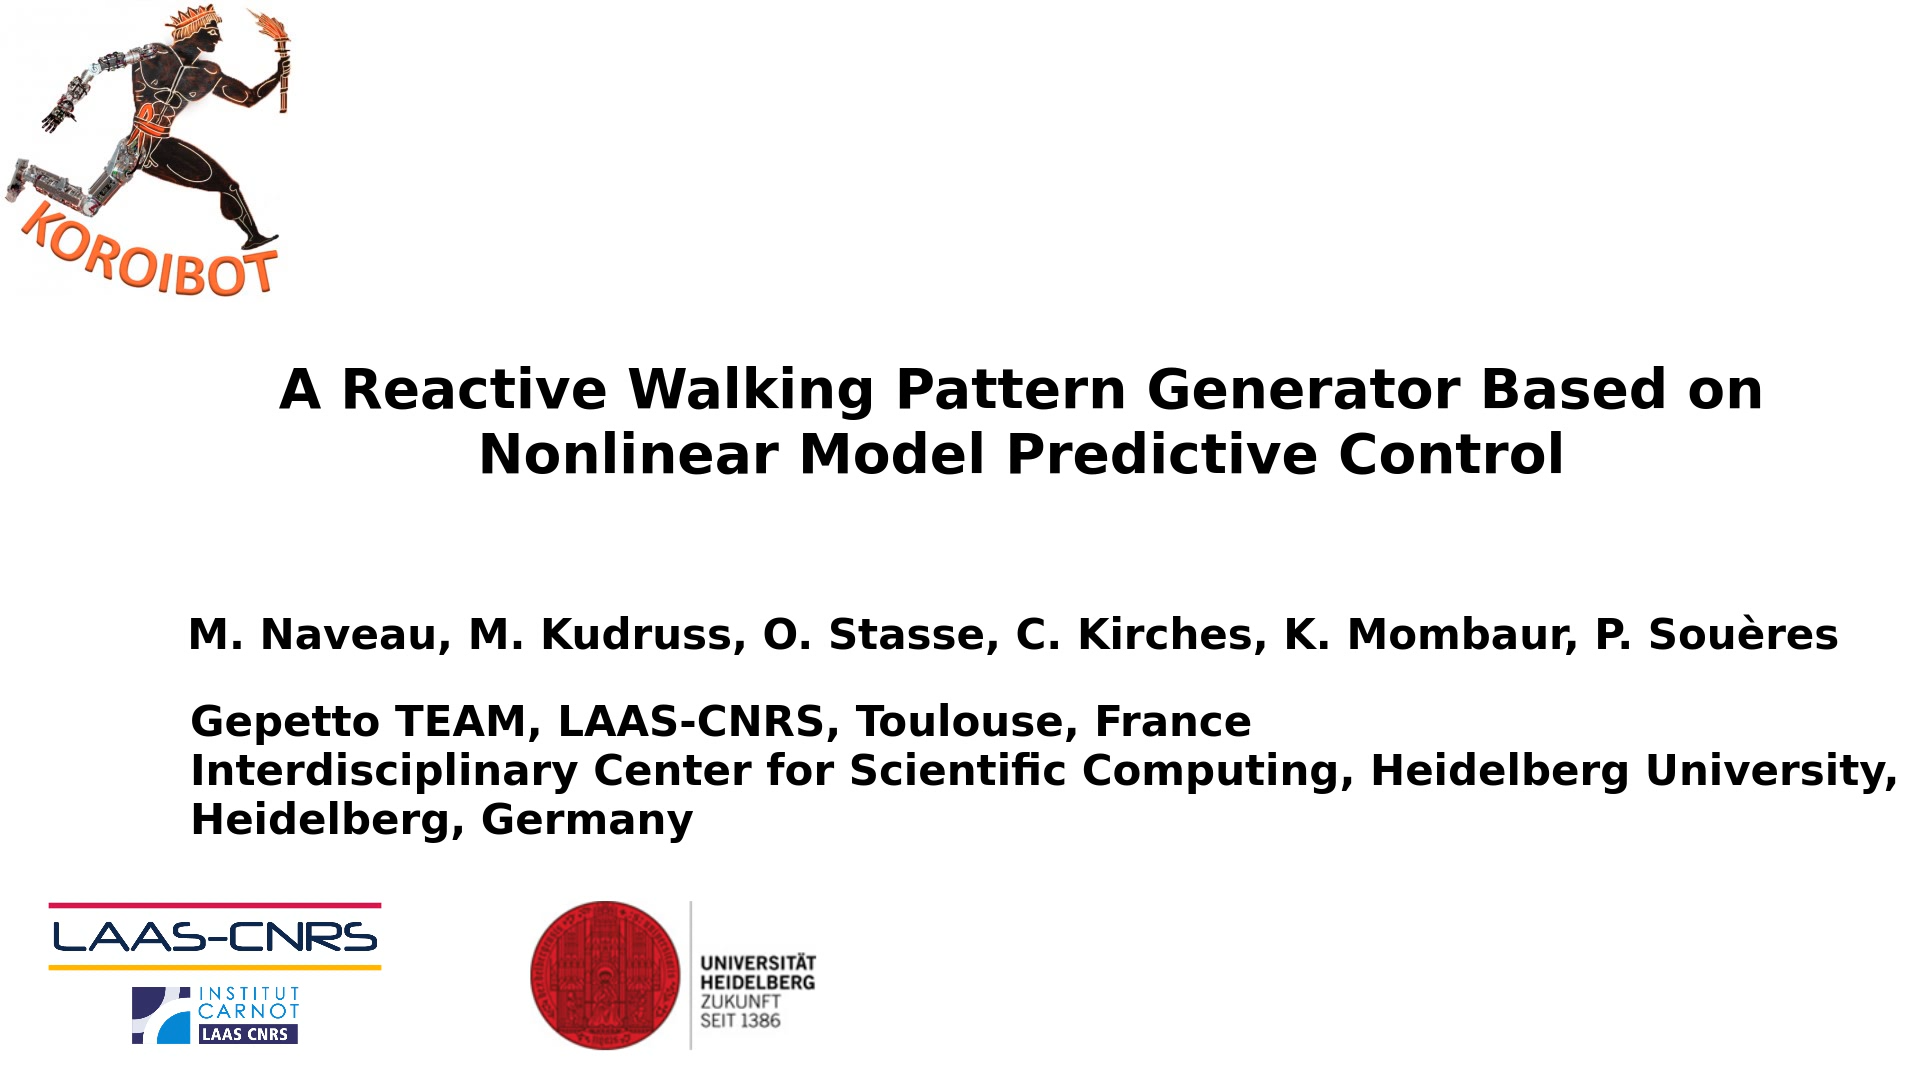
\includegraphics[width=0.85\linewidth, keepaspectratio]
      {16-raletter-NMPC-v19.png}    
    }  
    {videos/16-raletter-NMPC-short.mp4}
  \end{center}
  \vspace*{-0.5cm}
  \blfootnote{\textbf{Naveau}, Kudruss et al. RA-L 2016}
\end{frame}

%%%%%%%%%%%%%%%%%%%%%%%%%%%%%%%%%%%%%%%%%%%%%%%%%%%%%%%%%%%%%%%%%%%%%%%%%%%%%%%

